% ============================================================
% Mechanistic Validity: Scientific Formalization and Theory of
% Validity for Interpretability Claims
% ============================================================
\pdfoutput=1

\documentclass[10pt]{article}

\usepackage[margin=1in]{geometry}%
\usepackage{times}%
\usepackage{authblk}%

\usepackage[T1]{fontenc}
\usepackage[utf8]{inputenc}
\usepackage{microtype}
\usepackage{amsmath,amssymb}
\usepackage{booktabs}
\usepackage{graphicx}
\graphicspath{{figures/}}
\usepackage{xcolor}
\usepackage{hyperref}
\usepackage{cleveref}
\usepackage{enumitem}
\usepackage{placeins}
\usepackage{float}
\usepackage{multirow}
\usepackage{array}

% --- Macros ---
\newcommand{\mechval}{\textsc{MechVal}}
\newcommand{\ie}{i.e.}
\newcommand{\eg}{e.g.}
\newcommand{\cf}{cf.}

% tight tables
\newcommand{\tighttable}{\setlength{\tabcolsep}{4pt}\renewcommand{\arraystretch}{1.05}}

% add space between caption and table rule
\usepackage{caption}
\usepackage{natbib}
\captionsetup[table]{skip=8pt}

% fix appendix spacing
\title{Mechanistic Validity: A Theory of Validity for Interpretability Claims}
\author{Elliot Tower\\ Independent Researcher\\ \texttt{elliot@elliottower.ai}}


%\def\month{06}
%\def\year{2026}
%\def\openreviewid{ABC123XYZ}


\begin{document}

\maketitle

% ============================================================
\begin{abstract}
A mechanistic explanation of a neural network is not a single experimental result, but a structured claim linking a theoretical construct, a measurement procedure, an intervention, and a scope of interpretation. We introduce Mechanistic Validity (\mechval{}), a formalized epistemology for validating these causal claims, drawing on validation methodology from causal inference, measurement theory, and the philosophy of science. The framework makes interpretability claims explicit, falsifiable, and comparable, formalizing the discovery, validation, and interpretation of causal mechanisms as separate evidential stages. \mechval{} evaluates claims through six layers: (1) \emph{description mode}, (2) \emph{evidence family}, (3) \emph{metrics}, (4) \emph{criteria}, (5) \emph{validity type}, (6) \emph{verdict}. A gap at any layer is visible in the final verdict. The framework is method-agnostic, applying the same criteria to circuits, SAE features, probing classifiers, steering vectors, transcoders, and crosscoders. Applying the framework to 13 published circuits, we show that the tier system discriminates among claims---from Proposed (probing classifiers) to Triangulated (induction heads)---with every verdict traceable to specific present or missing evidence. By making the evidential status of a claim explicit and the path to strengthening it concrete, \mechval{} provides a foundation for interpretability claims that are explicit, testable, and scientifically grounded.
\end{abstract}

% ============================================================
\section{Introduction}
\label{sec:intro}

Mechanistic interpretability has produced a remarkable catalog of internal mechanisms:
induction heads that implement in-context copying \citep{olsson2022context}, a multi-role
circuit for indirect object identification \citep{wang2023interpretability}, a greater-than
algorithm \citep{hanna2023greater}, and sparse autoencoder features proposed to correspond
to human-interpretable concepts \citep{cunningham2023sparse, bricken2024monosemanticity}. The field has also begun to
build evaluation infrastructure: faithfulness metrics for circuits
\citep{miller2024transformer}, the Mechanistic Interpretability Benchmark for comparing
localization methods across tasks and models \citep{mueller2025mib}, SAEBench for auditing
sparse autoencoder quality \citep{karvonen2025saebench}, and causal scrubbing for testing
mechanistic hypotheses via behavior-preserving resampling \citep{chan2022causal}.

These contributions evaluate important objects---methods, circuits, features, alignments,
benchmark scores. They do not by themselves answer a different question: what has been
established by a mechanistic interpretability \emph{claim}? A claim such as ``this head is
a name mover,'' ``this feature represents deception,'' or ``this subspace implements a
causal variable'' is not just a circuit or a metric value. It links a theoretical
construct to a measurement procedure, a causal intervention, a scope of generalization,
and a natural-language interpretation. Shared metrics are not yet shared validity criteria.

A mechanistic narrative that was retrofitted to match ablation results is currently
indistinguishable from one that has survived refutation attempts. This matters because a
mechanistic explanation has many adjustable parts---which components to include, what roles
to assign, which edges to draw---and a narrative with enough flexibility will always fit
the observations. The \mechval{} framework introduced below provides the criteria needed to
distinguish well-supported claims from plausible-sounding ones, making the gaps in evidence
visible rather than leaving them implicit.

Several recent results sharpen this point. The SAEBench audit reveals that two of six
standard SAE evaluation metrics fail basic diagnostics for reseed stability, ground-truth
correlation, and discriminability \citep{karvonen2025saebench}. Execution-grounded
reproducibility checks via MechEvalAgent \citep{bai2026mecheval} surface claim-evidence
coherence issues that narrative review misses. And unconstrained nonlinear alignment maps can achieve 100\% interchange-intervention
accuracy on randomly initialized models \citep{sutter2025nonlinear}---not an impossibility
result for causal abstraction, but a worked example of what happens when measurement
validity is skipped. Each finding bears on a different link in the inference chain: measurement
reliability, reproducibility, and baseline separation, respectively. What is missing is
not any one fix but a principled way to ask, of any claim, which links have been
established and which have not.

The need for such a framework is not only academic.  A major coordinated funding signal in AI safety research---the Schmidt Sciences Trustworthy AI agenda \citep{schmidt2026trustworthy}---calls for construct validity, predictive validity, and cross-model generalization of interpretability findings, using precisely these terms but without a unified framework for operationalizing them.  The agenda asks whether mechanistic claims about deception, planning, and situational awareness can be trusted enough to inform deployment decisions.  \mechval{} provides the missing layer: a structured protocol that takes the validity vocabulary the field already uses informally and makes it operational, falsifiable, and auditable.

We introduce \mechval{}, a formalized epistemology for validating mechanistic interpretability claims, drawing on validation methodology from causal inference, measurement theory, and the philosophy of science. The framework evaluates claims through a six-layer pipeline: first, a \emph{description mode} declares at what level the claim is stated---computational, algorithmic, or implementational. Then \emph{evidence families} classify the kinds of signal available (causal, structural, behavioral, representational, information-theoretic, measurement). Concrete \emph{metrics} produce measurements, which are scored against 30 operational \emph{criteria} grouped into five \emph{validity types}---construct, measurement, internal, external, and interpretive---in dependency order. The result is a \emph{verdict}: a structured validity profile showing which criteria are met, which are untested, and which fail, with a tier from Proposed to Validated summarizing the overall evidential status.

The pipeline has two uses. When \emph{running experiments}, evidence builds upward from metrics through criteria to a verdict. When \emph{auditing a claim}, the process reverses: starting from a verdict, the framework identifies which criteria are unmet and whether the description mode is supported by the available evidence. Most published MI claims, when audited, land at Causally Suggestive or Mechanistically Supported---necessity is shown but specificity, measurement calibration, or cross-method consistency remain untested.

\mechval{} is claim-centric and method-agnostic: it evaluates circuits, SAE features, probing classifiers, steering vectors, transcoders, and crosscoders with the same criteria. It does not replace existing benchmarks or methods. It provides a common layer above them: claim-level validation built on method-level evaluation.

We describe the framework (\Cref{sec:framework}), its theoretical foundations (\Cref{sec:foundations}), its application to 13 published circuits (\Cref{sec:case-studies}), and its implications for the field (\Cref{sec:discussion}).

% ============================================================
\section{Related Work}
\label{sec:related}

\mechval{} is designed to complement, not replace, existing MI evaluation infrastructure. MIB \citep{mueller2025mib} is method-vs-method: which discovery algorithm produces the best circuit? TracR \citep{lindner2024interp} is method-vs-ground-truth: does the method find the true circuit in a synthetic model? \mechval{} is claim-centric: given a claim about how a model works, what evidence supports it and what remains untested? MIB and TracR evaluate discovery methods; \mechval{} evaluates the claims built on their outputs.

Recent work applies construct validity theory to ML evaluation more broadly. \citet{bean2025measuring} find that fewer than 16\% of LLM benchmarks use statistical validity methods, and \citet{freiesleben2025benchmarking} develop a psychometric framework for benchmark evaluation grounded in Cronbach, Meehl, and Messick. Both are benchmark-centric: they assess whether a benchmark measures what it claims to measure. \mechval{} extends this approach from benchmarks to mechanistic claims, and from construct validity alone to five distinct validity types in dependency order---construct, measurement, internal, external, and interpretive---each grounded in an established scientific tradition.

SAEBench \citep{karvonen2025saebench} audits SAE evaluation metrics; \mechval{} treats that audit as evidence about its own measurement-validity criteria (M1--M6). MechEvalAgent \citep{bai2026mecheval} checks whether published MI code reproduces; \mechval{} asks whether the evidence pattern supports the claim. Unstructured LLM-as-judge evaluation \citep{zheng2023judging} lacks the operational criteria to distinguish validity from plausibility. A companion paper automates \mechval{} via structured LLM extraction against the 30 criteria.



\begin{figure}[H]
\centering
\vspace{-4pt}
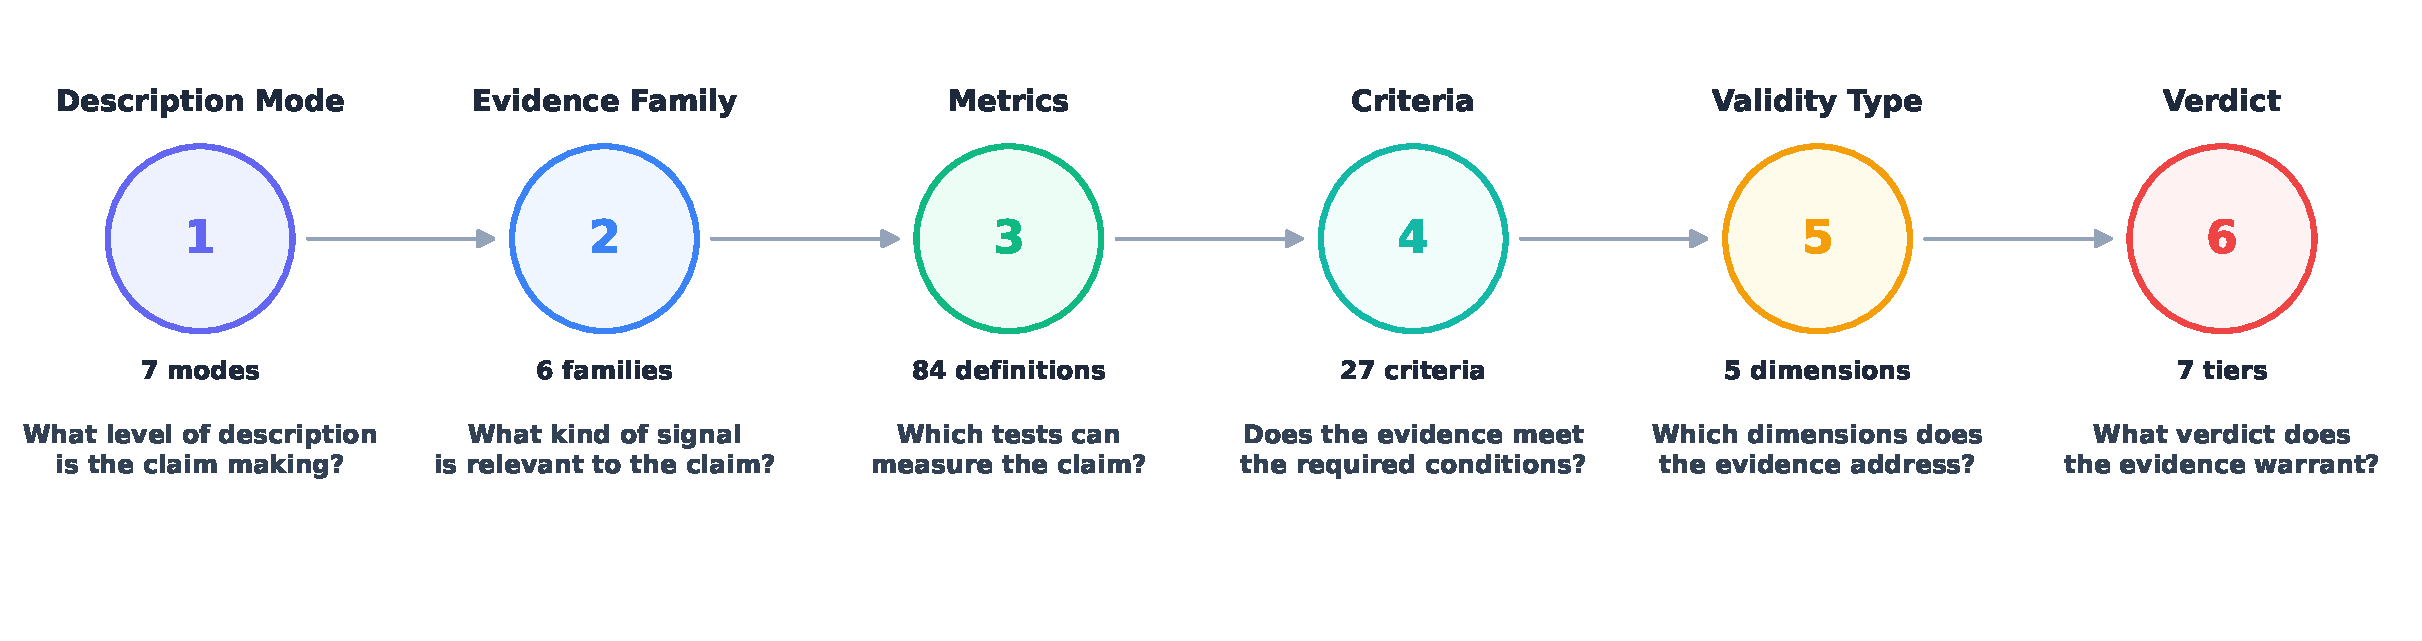
\includegraphics[width=\linewidth, trim=0 0 0 40, clip]{pipeline-F.pdf}
\vspace{-8pt}
\caption{The \mechval{} framework hierarchy. When running experiments, evidence builds upward from metrics through criteria to a verdict. When auditing a claim, the process reverses: starting from a verdict, the framework identifies which criteria are met and whether the description mode is supported by the available evidence.}
\label{fig:pipeline}
\end{figure}


% ============================================================
\section{From Claim to Verdict}
\label{sec:overview}

Consider a concrete claim: ``The IOI circuit uses three name-mover heads (9.9, 9.6, 10.0) to copy the indirect object to the output position.'' This claim appears in a widely-cited paper, is supported by ablation experiments, and has a clear mechanistic narrative. What has this claim established, and what remains untested?

The framework evaluates such a claim through six layers (\Cref{fig:pipeline}):

\begin{enumerate}[nosep]
\item \textbf{Description mode.} At what level is the claim made? The IOI claim operates at the implementational-functional level: it names specific heads and says what each one does. A weaker claim (``GPT-2 solves IOI'') would be computational; a stronger one (``head 9.9 implements copying via its OV circuit'') would require additional structural evidence.

\item \textbf{Evidence family.} What kinds of evidence are available? The original IOI paper provides primarily causal evidence (ablation) and some behavioral evidence (faithfulness). Structural evidence (weight-space analysis of the OV circuits) and cross-model evidence (does the same circuit appear in GPT-2 Medium?) would strengthen the claim by adding independent failure modes.

\item \textbf{Metrics.} Which concrete tests were run? Activation patching, role ablation, faithfulness scores. Each metric belongs to an evidence family and produces a measurement that feeds into criteria evaluation.

\item \textbf{Criteria.} Does the evidence meet the bar? The IOI circuit passes necessity (I1: ablation degrades performance) and sufficiency (I2: the circuit alone recovers 87\% of logit difference). But specificity (I3: does the circuit affect \emph{only} IOI?) is untested, and the 87\% faithfulness number is method-conditional---it drops below 50\% under non-mean-ablation methods \citep{miller2024transformer}, partially failing intervention reach (E1).

\item \textbf{Validity type.} Which validity dimensions are satisfied? Construct validity (the claim is well-defined), partial internal validity (necessity and sufficiency shown but specificity untested), partial external validity (limited prompt generalization, no cross-model replication). Measurement validity is unaddressed---no calibration of the ablation metrics themselves.

\item \textbf{Verdict.} What tier does the claim reach? Mechanistically Supported---necessity and sufficiency are established with at least one method, but the evidence comes primarily from one methodological family (ablation-based), key criteria remain untested (I3, I4, E4), and the faithfulness result is method-conditional. The verdict is not a judgment on the paper's quality; it is a precise characterization of what has been established and what has not.
\end{enumerate}

The 30 criteria also formalize common failure modes observed in published MI research (\Cref{tab:failures}).

\begingroup
\small
\begin{table}[H]
\centering
\caption{Twelve common failure modes in MI research, each mapped to the criteria that detect it.}
\label{tab:failures}
\renewcommand{\arraystretch}{1.15}
\begin{tabular}{@{}l>{\raggedright\arraybackslash}p{3.2cm}>{\raggedright\arraybackslash}p{2.8cm}>{\raggedright\arraybackslash}p{4.0cm}@{}}
\toprule
\textbf{Failure mode} & \textbf{What happens} & \textbf{Criterion} & \textbf{Example} \\
\midrule
Cherry-picking metrics & Run multiple ablation methods, report only the best number & E1 Intervention\newline reach & IOI: 87\% mean ablation reported; resample ablation (40\%) omitted \\
\midrule
No baseline control & Report high score without testing a random or untrained model & M2 Baseline\newline separation & Unconstrained nonlinear IIA achieves 95\% on random models; structured methods with identifiability constraints do not \citep{sutter2025nonlinear} \\
\midrule
No negative controls & Only test predictions that should pass; never test what the mechanism should \emph{not} affect & I3 Specificity\newline C1 Falsifiability & Successor heads: cross-domain ablation effects on non-successor tasks never reported \\
\midrule
Construct incoherence & Target construct is not separable from a neighboring one & C4 Discriminant\newline validity & Gender bias circuits: bias and knowledge share the same heads \\
\midrule
Off-target effects & Ablation works for the target task; other tasks never checked & I3 Specificity & Knowledge neurons: editing one fact corrupts related facts (ripple effects) \\
\midrule
Circuit redefinition & Drop heads that hurt faithfulness, call it ``refined'' & C1 Falsifiability & Adjusting circuit membership to maximize the target metric \\
\midrule
Post-hoc role labeling & Name heads after observed behavior; the label cannot fail & C1 Falsifiability & ``Name mover'' assigned after seeing logit attribution \\
\midrule
No double dissociation & Show necessity but never test the converse & I4 Double\newline dissociation & IOI circuit ablated $\to$ IOI breaks; SVA circuit $\to$ IOI intact never tested \\
\midrule
Interpretive inflation & Label implies intent or algorithm beyond what evidence shows & V4 Anthropo-\newline morphism check & ``World model'' for Othello (evidence supports ``linearly decodable'') \\
\midrule
Scope creep & Validate on one prompt format, claim generality & V5 Scope decl.\newline E2 Prompt gen. & Greater-than circuit tested only on year ranges; claimed as general ordinal comparison \\
\midrule
Flexible scope & Narrow the claim after seeing results so it cannot fail & V5 Scope\newline declaration & Restricting scope post-hoc to the subset of prompts that work \\
\midrule
Ignoring alternatives & Circuit works, but so does a different set of heads & I4 Double dissoc.\newline C3 Convergent val. & Meloux et al.\ find alternative IOI circuits with comparable faithfulness \\
\bottomrule
\end{tabular}
\end{table}
\endgroup


% ============================================================
\section{The Framework}
\label{sec:framework}


The \mechval{} framework has six layers, presented here in pipeline order (\Cref{fig:pipeline}): description modes (\Cref{sec:description-modes}), evidence families (\Cref{sec:evidence-families}), metrics (\Cref{sec:metrics}), criteria (\Cref{sec:criteria}), validity types (\Cref{sec:validity-types}), and verdict tiers (\Cref{sec:verdict-tiers}).

\subsection{Description Modes}
\label{sec:description-modes}

A description mode is a commitment about what kind of explanation is being offered (\Cref{tab:modes}). It is not a label applied after analysis---it is a declaration that determines what counts as evidence, what counts as a gap, and what the finding means if it succeeds. The distinction matters because mechanistic interpretability routinely conflates levels: a paper that discovers \emph{which components} are active (implementational-topographic) writes a narrative about \emph{what the model computes} (computational). Each level upgrade requires additional bridging evidence that the lower level cannot provide.

The seven modes, adapted from Marr's hierarchy \citep{marr1982vision}, form a partial order by evidential commitment. A computational claim commits to a function being computed and a reason it is the right function. An algorithmic claim commits to a specific procedure. A representational claim commits to what information is encoded but not how it is processed. The four implementational sub-types commit to progressively weaker structural facts: which components are involved (topographic), how they are wired (connectomic), what their activations look like (statistical), and what input-output transformation each performs (functional).

\begin{table}[H]
\centering
\small
\caption{Seven description modes, ordered from most committal (computational) to least committal (topographic). Higher modes require all evidence from lower modes plus bridging evidence. Implementational-statistical is partially orthogonal: it characterizes activation distributions rather than making structural commitments.}
\label{tab:modes}
\renewcommand{\arraystretch}{1.2}
\begin{tabular}{@{}rl>{\raggedright\arraybackslash}p{4.8cm}>{\raggedright\arraybackslash}p{5.2cm}@{}}
\toprule
& \textbf{Mode} & \textbf{What it asks} & \textbf{Example} \\
\midrule
1 & Computational & What function does the system compute, and why? & ``GPT-2 predicts the indirect object'' \\
\midrule
2 & Algorithmic & What procedure does it execute? & ``A detect-inhibit-copy algorithm'' \\
\midrule
3 & Representational & What information is encoded, and in what geometry? & ``The IO name is linearly encoded at layer 8'' \\
\midrule
4 & Impl.-Functional & What transformation does each component perform? & ``Head 9.9 copies names to the output'' \\
\midrule
5 & Impl.-Connectomic & How are components wired? & ``S-inhibition feeds name movers via residual stream'' \\
\midrule
6 & Impl.-Statistical & What do activations look like? & ``Head 9.9 attends strongly to IO position'' \\
\midrule
7 & Impl.-Topographic & Which components are involved? & ``Heads 9.9, 9.6, 10.0'' \\
\bottomrule
\end{tabular}
\end{table}

A claim may carry evidence at several modes simultaneously; the framework does not average them. Each mode-level sub-claim receives its own assessment, and the overall verdict is reported at the strongest mode whose required evidence is complete, with lower-mode evidence noted as supporting and higher-mode evidence as suggestive. The mode assigned to a verdict is thus the strongest level for which all required evidence is present. Partial evidence at a higher level does not upgrade the mode---it is reported as suggestive while the verdict is issued at the established mode. For example, a claim at the algorithmic level (``the model runs a detect-inhibit-copy algorithm'') requires both the topographic evidence (which heads are involved) and the additional evidence that the heads implement the claimed procedure---path-level causal tracing, timing consistency, and sufficiency of the minimal circuit.

\subsection{Evidence Families}
\label{sec:evidence-families}

An evidence family classifies a metric's output by the kind of signal it produces, independent of the specific tool used to generate it (\Cref{tab:families}). The classification matters because convergent validity---two independent lines of evidence agreeing---is the strongest form of support for a mechanistic claim. But not all agreement is equally informative: two causal metrics agreeing shares failure modes, while a causal ablation and a representational probe agreeing is substantially stronger, because convergent evidence provides triangulated support across independent methodologies.

\begin{table}[H]
\centering
\small
\caption{Six evidence families. Convergent evidence across families with independent failure modes is qualitatively stronger than redundant evidence from the same family.}
\label{tab:families}
\renewcommand{\arraystretch}{1.2}
\begin{tabular}{@{}ll>{\raggedright\arraybackslash}p{4.5cm}>{\raggedright\arraybackslash}p{5cm}@{}}
\toprule
& \textbf{Family} & \textbf{What it measures} & \textbf{Examples} \\
\midrule
A & Causal & Effects of interventions on computation & Activation patching, DAS-IIA, CATE, mediation \\
\midrule
B & Structural & Weight-space properties (no forward pass) & SVD, effective rank, OV/QK composition \\
\midrule
C & Information & Information flow and dependencies & Mutual information, PID, OCSE, transfer entropy \\
\midrule
D & Behavioral & Input-output behavior under manipulation & Faithfulness, logit diff, KL divergence, dose-response \\
\midrule
E & Representational & Geometry of internal representations & CKA, RSA, linear probes, attention entropy \\
\midrule
F & Measurement & Trustworthiness of other metrics & Bootstrap stability, seed variance, convergent validity \\
\bottomrule
\end{tabular}
\end{table}

The primary function of the family classification is to structure convergent validity assessments. When evaluating a claim, the analyst asks three questions: How many evidence families support the claim? Which families are represented? And are there families that \emph{should} support the claim but do not? Absence of expected evidence from a family is informative: it may indicate a gap in the claim or a limitation of the proposed mechanism.

Each family answers a different question. Causal metrics ask: does this component matter for this behavior? Structural metrics ask: what does the architecture encode before any data flows? Behavioral metrics ask: does the proposed circuit actually produce the behavior it is supposed to explain? Representational metrics ask: what does this component represent? Information-theoretic metrics ask: how much does this component know about the task variable? And measurement metrics ask: can the other metrics' outputs be trusted?

Each family has characteristic strengths and blind spots. Causal metrics (A) establish necessity and sufficiency directly but are vulnerable to backup circuits that compensate after ablation. Structural metrics (B) cannot be confounded by runtime compensation but cannot distinguish used capacity from unused capacity. Behavioral metrics (D) test whether the circuit reproduces the model's outputs, but behavioral equivalence does not imply mechanistic equivalence---different circuits can produce the same behavior for different reasons. Measurement metrics (F) are uniquely important because they evaluate the other families' outputs: a reliable metric pointed at the wrong target produces confident wrong answers.

\subsection{Metrics}
\label{sec:metrics}

Metrics are concrete, runnable tests that produce measurements about a neural network---the layer of the hierarchy where empirical contact with the model actually happens. Everything above (evidence families, criteria, validity types, verdicts) depends on what metrics measure and how well they measure it. A metric alone cannot establish a claim; a claim requires evidence from multiple metrics, evaluated against the criteria appropriate to the validity type being asserted.

Each metric takes a model, a task, and optionally an intervention as input, and produces a number as output. Metrics can be composed: one metric's output feeds into another. The 14 calibrations in family F are meta-metrics---they take another metric's output as input and assess whether it is stable (bootstrap stability), reproducible (seed variance), or distinguishable from baselines (baseline separation). A high score on a primary metric is not evidence if the corresponding calibration fails. The framework organizes evidence into six metric families; the current catalog enumerates 84 metric definitions across families A--E; \Cref{tab:causal_metrics} illustrates the causal family. The full inventory for all six families is in \Cref{appendix:metrics}.

\begin{table}[H]
\centering
\small
\caption{Causal metrics (family A): effects of interventions on model computation.}
\label{tab:causal_metrics}
\renewcommand{\arraystretch}{1.15}
\begin{tabular}{@{}l>{\raggedright\arraybackslash}p{9.5cm}@{}}
\toprule
\textbf{Metric} & \textbf{Description} \\
\midrule
A01 SCM / Pearl & Structural causal models and do-calculus as the formal language for circuit claims \\
\midrule
A02 Counterfactual DAS & Distributed Alignment Search and IIA for testing causal abstraction hypotheses \\
\midrule
A03 Rubin CATE & Conditional average treatment effects across input subpopulations \\
\midrule
A04 Woodward & Interventionist theory of causation applied to circuit ablation \\
\midrule
A05 MDC / Glennan & New mechanical philosophy: components organized to produce phenomena \\
\midrule
A06 Mediation & Natural direct and indirect effects decomposition for circuit paths \\
\midrule
A07 Granger / TE & Observational causal discovery via conditional MI and temporal precedence \\
\midrule
A08 PID & Decomposing MI into redundant, unique, and synergistic contributions \\
\midrule
A09 MDL / SLT & Minimum description length and singular learning theory for circuit complexity \\
\midrule
A10 Regularity / INUS & INUS conditions: insufficient but necessary parts of sufficient sets \\
\midrule
A11 Actual Cause & Halpern-Pearl actual causation on specific inputs, not just potential causes \\
\midrule
A12 Transportability & Formal conditions for circuit generalization across models and distributions \\
\midrule
A13 Causal Discovery & NOTEARS / PC algorithms for learning DAGs over circuit components \\
\bottomrule
\end{tabular}
\end{table}

The causal family draws on multiple distinct traditions of causation, each formalized as a metric. \emph{Interventionist frameworks} (Pearl's SCM, Rubin's potential outcomes, Woodward's interventionism, Geiger et al.'s DAS) formalize what happens when components are ablated or patched. \emph{Information-theoretic approaches} (Granger causality, partial information decomposition) measure directed information flow without requiring explicit interventions. \emph{Structural approaches} (mediation analysis, INUS conditions, Halpern-Pearl actual causation, singular learning theory) characterize the causal graph itself---its paths, its minimal sufficient sets, and its complexity. And \emph{generalization approaches} (Pearl and Bareinboim's transportability, constraint-based discovery algorithms like PC and NOTEARS) address whether causal findings transfer across settings and whether circuit distinction can be learned from observational data.


Many metrics correspond to entire experimental methodologies in their source fields; the framework represents them as metrics to provide a common unit of comparison across evidence families and allow them to be scored against the same criteria. Some concepts appear in multiple families because they serve different evidential roles in each: Granger causality appears in family A (as a causal metric testing directed influence via interventions) and family C (as an information-theoretic metric quantifying observational information flow); partial information decomposition appears in family A (decomposing causal contributions) and family C (decomposing mutual information). The family assignment reflects the evidential question the metric answers in that context, not the mathematical formalism.

\subsection{Criteria}
\label{sec:criteria}

Criteria are specific, falsifiable conditions that must be met for a validity type to be satisfied (\Cref{tab:criteria}). Each criterion has a concrete pass condition---for example, I1 (necessity) requires that ablating the component degrades performance across at least two independent methods, not just one. A claim either passes, partially passes, or fails each criterion, producing a structured validity profile rather than a single score.

\begingroup
\hyphenpenalty=10000
\exhyphenpenalty=10000
\begin{table}[H]
\centering
\small
\caption{Thirty criteria across five validity types. Each criterion has a concrete test; a claim either passes, partially passes, or fails, producing a structured validity profile.}
\label{tab:criteria}
\renewcommand{\arraystretch}{1.15}
\begin{tabular}{@{}llp{8.5cm}@{}}
\toprule
\textbf{ID} & \textbf{Criterion} & \textbf{Description} \\
\midrule
C1 & Falsifiability & Can the claim be refuted? \\
C2 & Structural plausibility & Is the mechanism physically possible in the architecture? \\
C3 & Convergent validity & Do multiple independent methods agree? \\
C4 & Discriminant validity & Does the measure distinguish this from neighboring constructs? \\
C5 & Nomological validity & Does the claim fit into a broader theory? \\
\midrule
M1 & Reliability & Do repeated measurements give the same answer? \\
M2 & Baseline separation & Is the score distinguishable from random/untrained baselines? \\
M3 & Stability & Is the classification robust to perturbation? \\
M4 & Calibration & Are the numbers meaningful? \\
M5 & Sensitivity & Can the instrument detect known-true effects? \\
M6 & Invariance & Does the metric behave consistently across conditions? \\
\midrule
I1 & Necessity & Is the circuit required for the behavior? \\
I2 & Sufficiency & Is the circuit enough to produce the behavior? \\
I3 & Specificity & Does the circuit do this task and not everything? \\
I4 & Double dissociation & Can this circuit be separated from other circuits? \\
I5 & Confound control & Are alternative explanations ruled out? \\
I6 & Epistatic interaction & Do circuit components interact non-additively? \\
I7 & Rescue reversibility & Does restoring a corrupted component recover behavior? \\
I10 & Confounding sensitivity & How strong must an unmeasured confounder be to explain the result? \\
\midrule
E1 & Intervention reach & Do different intervention methods agree? \\
E2 & Prompt generalization & Does it work on diverse prompts? \\
E3 & Cross-task generalization & Does the mechanism transfer to related tasks? \\
E4 & Cross-model generalization & Does the mechanism appear in other models? \\
E5 & Graded response & Does partial ablation produce partial effects? \\
E6 & Novel prediction & Does the mechanism predict new, untested behaviors? \\
\midrule
V1 & Level declaration & At what description mode is the claim made? \\
V2 & Level-evidence match & Does the evidence support claims at that level? \\
V3 & Alternative level & Could the evidence be explained at a different level? \\
V4 & Anthropomorphism check & Is the interpretation projecting human concepts? \\
V5 & Scope declaration & What does the claim explicitly not cover? \\
\bottomrule
\end{tabular}
\end{table}
\endgroup




\begingroup
\hyphenpenalty=10000
\exhyphenpenalty=10000
\begin{table}[H]
\centering
\small
\caption{Criterion status categories. Status labels summarize the evidential state of an individual criterion, not the overall verdict for the claim.}
\label{tab:criterion-status}
\renewcommand{\arraystretch}{1.15}
\begin{tabular}{@{}lp{10.5cm}@{}}
\toprule
\textbf{Status} & \textbf{Meaning} \\
\midrule
Confirmed & Tests capable of exposing the relevant failure mode were conducted and passed. \\
\midrule
Partially confirmed  & Supportive evidence exists, but it is too narrow, method-dependent, weakly calibrated, or insufficiently severe to establish the criterion. \\
\midrule
Inconclusive & Relevant tests give conflicting results across methods, datasets, interventions, calibrations, or scopes. \\
\midrule
Disconfirmed & An appropriate test was conducted and the criterion failed. \\
\midrule
Untested & No test capable of evaluating the criterion has been conducted. \\
\bottomrule
\end{tabular}
\end{table}
\endgroup

For each validity criterion, we assign a criterion status from an ordered five-level scale: Confirmed, Partially confirmed, Inconclusive, Disconfirmed, or Untested. These statuses are ordinal verdict categories in the error-statistical tradition of \citet{mayo1996error, mayo2018statistical}: a criterion is Confirmed if and only if the relevant experimental tests were conducted under conditions of sufficient severity to have detected failure, and the criterion passed those tests. Following \citet{achinstein2001book}, we further distinguish criteria where the available evidence constitutes a genuine epistemic reason to accept the criterion (Confirmed) from those where evidence is present but falls short of that bar (Partially confirmed, Inconclusive). This framework is non-probabilistic: status assignments do not represent posterior beliefs or confidence levels. Instead, following \citet{campbell1963experimental} and \citet{cook1979quasi}, validity claims are evaluated by whether the relevant tests rule out plausible rival explanations. The Untested status applies when no test capable of evaluating the criterion has been conducted, whereas Inconclusive indicates contested evidence and Disconfirmed indicates that a test was conducted and the criterion failed.


These statuses evaluate individual criteria, not the overall claim. A claim can therefore contain Confirmed internal-validity criteria, Untested measurement-validity criteria, and Mixed external-validity criteria while still receiving a single overall verdict tier. This keeps criterion-level strengths, gaps, and failures explicit instead of compressing them into an undifferentiated verdict.

\subsection{Validity Types}
\label{sec:validity-types}

The five validity types form a dependency chain \citep{shadish2002experimental}: later types cannot be established without first satisfying earlier ones. The ordering reflects logical precedence: a construct that is not well-defined cannot be reliably measured, an unreliable measurement cannot support a causal claim, a causal claim in one setting cannot be generalized, and an interpretation cannot be evaluated until the underlying evidence is characterized.

\begin{equation}
\text{Construct} \rightarrow \text{Measurement} \rightarrow \text{Internal} \rightarrow \text{External} \rightarrow \text{Interpretive}
\label{eq:dependency}
\end{equation}

The pipeline (\Cref{fig:pipeline}) is procedural---it describes how evidence is built or audited. The validity-type chain is logical---it describes which types presuppose which. At pipeline step 5 (validity type), the framework evaluates every validity type the claim asserts, but the dependency order constrains the verdict: a claim cannot be credited with external validity beyond the level its measurement and internal validity support. The chain is a ceiling, not a sequence of gates.

Each type addresses a distinct question about the claim:

\paragraph{Construct validity.} Is the thing being measured well-defined? Before any measurement is taken, the construct must be specified precisely enough that the claim is falsifiable, structurally plausible, and distinguishable from neighboring constructs. A ``deception feature'' that cannot be distinguished from an ``uncertainty feature'' fails construct validity regardless of how carefully it is measured. This draws on philosophy of science (Popper's falsifiability, Hempel's operationalism) and psychometrics (construct validity, convergent and discriminant validity).

\paragraph{Measurement validity.} Are the instruments trustworthy? \citet{borsboom2004concept} argue that a measure is valid if and only if the attribute exists and variation in it causally produces variation in the measurement outcome. This causal account grounds the framework's measurement criteria. Once the construct is defined, the measurement tools used to detect it must be reliable (stable across repetitions), calibrated (separable from random baselines), and invariant (consistent across conditions). A metric that gives different answers when run with different random seeds is not evidence. This draws on psychometrics (test-retest reliability, measurement invariance) and pharmacology (assay validation).

\paragraph{Internal validity.} Does the evidence support the causal claim? Given a well-defined construct and trustworthy instruments, the evidence must establish that the identified component is causally involved in the behavior---not merely correlated with it. This requires demonstrating necessity (the component is required), sufficiency (the component is enough), and specificity (the component does this task and not everything). This draws on neuroscience (lesion studies, optogenetics, double dissociation) and causal inference \citep{pearl2009causality}.

\paragraph{External validity.} Does the mechanism generalize? Causal evidence on one prompt set, with one ablation method, in one model, establishes internal validity at best. External validity requires that the mechanism generalizes across prompts, ablation methods, related tasks, and ideally across models. This draws on pharmacology (Phase~III generalization, dose-response) and causal inference (transportability; \citealp{pearl2011transportability}).

\paragraph{Interpretive validity.} Is the interpretation of the mechanism correct? Finally, the natural-language description of the mechanism must be justified by the evidence. A head called a ``name mover'' based on direct logit attribution carries theoretical implications beyond what the evidence strictly supports. Interpretive validity requires declaring the description level, matching evidence to that level, and checking for anthropomorphic inflation. This draws on Messick's unified theory of validity \citep{messick1995validity}---which frames validity as the warrant for \emph{interpretations} of scores, not properties of the test itself---and on Marr's levels of analysis \citep{marr1982vision}.

\subsection{Verdict Tiers}
\label{sec:verdict-tiers}

Claims are assigned to one of five verdict tiers representing qualitative transitions in evidential status (\Cref{tab:verdicts}). Two additional labels---Underdetermined and Disconfirmed---handle special cases. The tiers form a strict hierarchy: each requires all evidence from the tier below plus additional evidence.

\begin{table}[H]
\centering
\tighttable
\caption{Verdict tiers with requirements. Each tier subsumes the requirements of all lower tiers.}
\label{tab:verdicts}
\small
\begin{tabular}{@{}lp{4.5cm}p{5.5cm}@{}}
\toprule
\textbf{Tier} & \textbf{Meaning} & \textbf{Requirements beyond previous tier} \\
\midrule
Proposed & Structural or representational evidence only & Construct validity criteria met (C1--C5) \\
\midrule
Causally Suggestive & Necessity shown, sufficiency not established & Internal validity I1 (necessity via ablation) \\
\midrule
Mechanistically Supported & Necessity + sufficiency with consistent methods & I1 + I2 (sufficiency), intervention reach (E1), at least 2 ablation variants \\
\midrule
Triangulated & Multiple converging lines of independent evidence & Full internal + external + construct criteria from $\geq 3$ evidence families \\
\midrule
Validated & All five validity types addressed & Measurement + interpretive validity with explicit baselines \\
\midrule
Underdetermined & Evidence consistent with multiple mechanisms & Cannot resolve between rival specifications \\
\midrule
Disconfirmed & Fails decisively on a key criterion & Negative result \\
\bottomrule
\end{tabular}
\end{table}

Every tier carries a specific epistemic meaning: a claim at \emph{Proposed} is not a failed claim but one whose evidential status---and the path to strengthening it---is precisely characterized. The verdict tells researchers exactly what additional evidence would advance the claim: a Proposed claim needs causal intervention (I1) to reach Causally Suggestive; a Causally Suggestive claim needs sufficiency evidence (I2) and method consistency (E1) to reach Mechanistically Supported.

Underdetermined and Disconfirmed serve distinct purposes. Underdetermined means the evidence is consistent with multiple competing mechanisms and the framework cannot resolve between them---this is not a lack of evidence but an excess of explanations, requiring additional experiments that discriminate between rivals. Disconfirmed means a criterion has been decisively failed---for example, when the construct itself turns out to be incoherent (C4), as in the gender bias circuits case study.



% ============================================================
\section{Theoretical Foundations}
\label{sec:foundations}

This section outlines the theoretical foundations of our framework. We draw on seven disciplines that each developed rigorous standards for a different validity question, and we apply them to mechanistic interpretability as lenses. A lens is not a method or a metric; it is an analytical vocabulary that shapes which questions you ask of a claim and how you read the answers. Each of the seven --- philosophy of science, psychometrics, causal inference, neuroscience, pharmacology, molecular genetics, and mechanistic interpretability itself --- contributes the conditions it requires before an inference is accepted, and names the failure modes it guards against.


\begin{figure}[H]
\centering
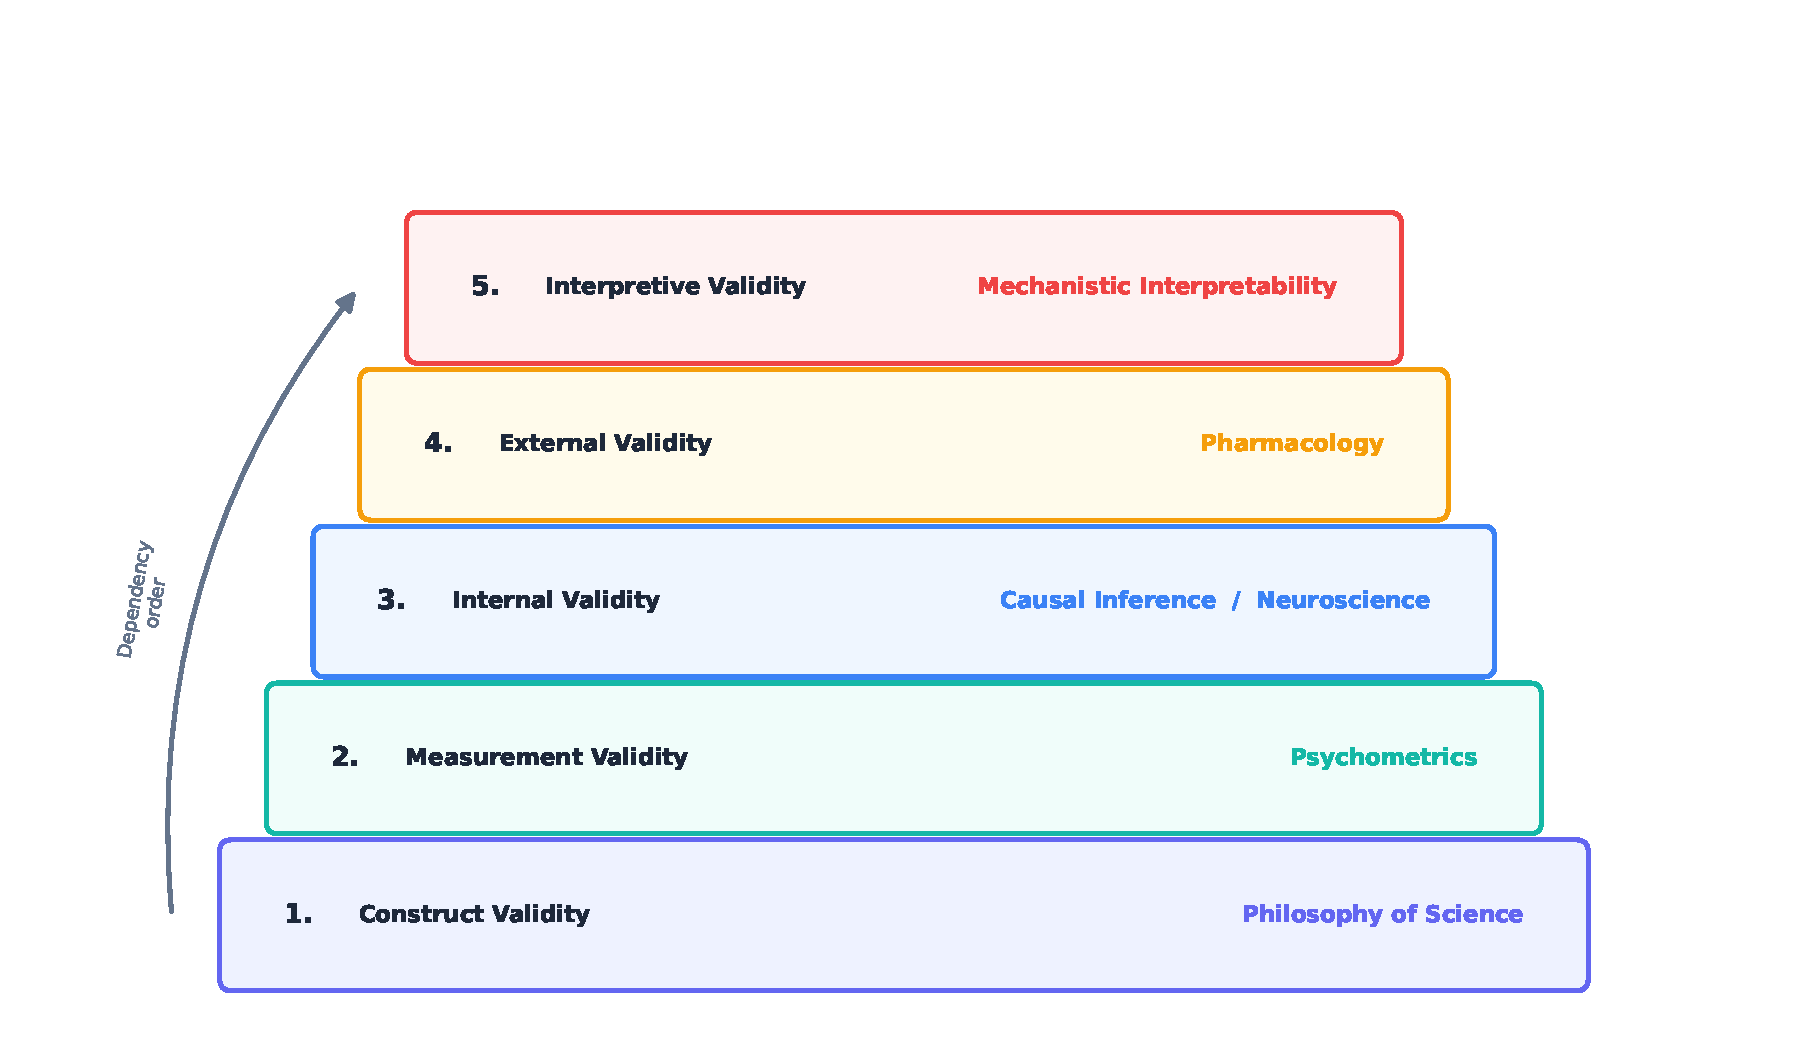
\includegraphics[width=\linewidth, trim=0 30 0 0, clip]{foundations-pyramid.pdf}
\caption{Seven theoretical foundations, each grounding a specific validity type. Causal inference, neuroscience, and molecular genetics all contribute to internal validity through complementary approaches (formal frameworks, experimental designs, and interaction structure, respectively).}
\label{fig:foundations}
\end{figure}

Each lens maps to a corresponding validity type, and answers a core question about a given claim: philosophy of science asks \emph{is the construct well-defined?} Causal inference and neuroscience ask \emph{does the component implement the computation?} Psychometrics asks \emph{is the measurement accurate?} Pharmacology asks \emph{does it generalize?} And mechanistic interpretability asks \emph{does the interpretation match the evidence?}

\subsection{Philosophy of Science}
\label{sec:phil-sci}

The construct validity criteria (C1--C5) draw on Popper's falsifiability criterion, Mayo's severe testing \citep{mayo2018statistical}, and Glennan's new mechanical philosophy \citep{glennan2017new}. A key distinction is between \emph{confirmation} and \emph{corroboration}: a circuit discovered by activation patching and evaluated by activation patching has only been shown to pass the test it was built to pass. Corroboration requires a genuinely risky test the circuit was not optimized for---a behavioral prediction on held-out prompts, a weight-space analysis, a different causal method. The verdict tier system reflects this hierarchy: single-method evidence (Causally Suggestive) is qualitatively weaker than convergent evidence from independent methods (Triangulated).

C5 (nomological validity) requires that the claim fit into a broader theoretical network, following Cronbach and Meehl's nomological network concept. The Duhem-Quine underdetermination problem is directly relevant: multiple circuits with low overlap can each individually pass faithfulness tests, and reporting this explicitly is a stronger finding than suppressing it.

\begin{table}[H]
\centering\small
\caption{Philosophy of science foundations.}
\renewcommand{\arraystretch}{1.12}
\begin{tabular}{@{}l>{\raggedright\arraybackslash}p{2cm}l>{\raggedright\arraybackslash}p{4.5cm}@{}}
\toprule
\textbf{Concept} & \textbf{Source} & \textbf{Criterion} & \textbf{MI analog} \\
\midrule
Falsifiability & \citet{popper1959logic} & C1 & What evidence would refute ``this is a name mover''? \\
\midrule
Nomological network & \citet{cronbach1955construct} & C5 & Does the claim connect to in-context learning theory? \\
\midrule
MTMM matrix & \citet{campbell1959convergent} & C3, C4 & Convergent: probing + patching agree. Discriminant: feature $\neq$ neighboring feature \\
\midrule
Underdetermination & \citet{duhem1906theorie} & I4 & Multiple circuits explain the same behavior \\
\midrule
Severe testing & \citet{mayo2018statistical} & C1 & A test that could easily have failed but did not \\
\bottomrule
\end{tabular}
\end{table}

\subsection{Psychometrics}
\label{sec:psychometrics}

The measurement validity criteria (M1--M6) draw on psychometric test construction. Classical test theory decomposes an observed score into true score plus error ($X = T + E$); M1 (reliability) is the proportion of true-score variance. Generalizability theory extends this by decomposing error into distinct sources---prompt variation, random seed, checkpoint selection---each of which can be quantified and reduced independently.

\begin{table}[H]
\centering\small
\caption{Psychometrics foundations.}
\renewcommand{\arraystretch}{1.12}
\begin{tabular}{@{}l>{\raggedright\arraybackslash}p{2.2cm}l>{\raggedright\arraybackslash}p{4.5cm}@{}}
\toprule
\textbf{Concept} & \textbf{Source} & \textbf{Criterion} & \textbf{MI analog} \\
\midrule
Classical test theory & \citet{lord1968statistical} & M1 & Same metric, same model $\to$ same answer \\
\midrule
Generalizability theory & \citet{cronbach1972dependability} & M6 & Decompose variance into prompt/seed/checkpoint \\
\midrule
Signal detection ($d'$) & \citet{green1966signal} & M2 & Is the score distinguishable from random? \\
\midrule
MTMM matrix & \citet{campbell1959convergent} & C3, C4 & Convergent + discriminant validity \\
\midrule
Selectivity & \citet{hewitt2019designing} & I3 & Probe accuracy minus control accuracy \\
\bottomrule
\end{tabular}
\end{table}

An important insight is that a reliable metric pointed at the wrong target produces confident wrong answers. \citet{sutter2025nonlinear} demonstrated that unconstrained nonlinear IIA achieves near-perfect scores on randomly initialized models---but this is a property of the \emph{unconstrained} alignment map, not of nonlinear causal abstraction in general. Structured generative models that satisfy identifiability conditions \citep{khemakhem2020variational}---reconstruction objectives, label-conditional priors, sparsity constraints---provably avoid this degeneracy: intervention diversity ratios near 1.0 confirm that the encoder preserves natural variation rather than collapsing to a lookup table. The framework addresses the general problem through M2 (baseline separation): not ``IIA = 0.48'' but ``$\Delta_{\text{random}} = 0.10$, $\Delta_{\text{untrained}} = 0.15$.'' A modest absolute number with a large delta is a genuine finding; a large absolute number with a tiny delta is not. The SAEBench audit \citep{karvonen2025saebench} provides a complementary example: two of six standard SAE evaluation metrics fail baseline separation entirely, producing scores on shuffled or random baselines that are indistinguishable from scores on real features.


\subsection{Causal Inference}
\label{sec:causal}

The internal validity criteria draw on causal inference methodology \citep{pearl2009causality, spirtes2000causation}. The necessity/sufficiency distinction maps to Woodward's interventionist causation \citep{woodward2003making}: necessity (I1) corresponds to ``would the behavior persist if the component were absent?'' and sufficiency (I2) to ``would the component alone produce the behavior?'' Pearl and Bareinboim's transportability theory \citep{pearl2011transportability} provides the formal conditions under which causal findings transfer across settings, grounding E4 (cross-model generalization). Rubin's potential outcomes framework grounds E5 (graded response) by formalizing heterogeneous treatment effects across input subpopulations---not all prompts may respond to ablation equally.

\begin{table}[H]
\centering\small
\caption{Causal inference foundations.}
\renewcommand{\arraystretch}{1.12}
\begin{tabular}{@{}l>{\raggedright\arraybackslash}p{2.5cm}l>{\raggedright\arraybackslash}p{4.2cm}@{}}
\toprule
\textbf{Concept} & \textbf{Source} & \textbf{Criterion} & \textbf{MI analog} \\
\midrule
do-calculus / SCM & \citet{pearl2009causality} & I1, I2 & Formal language for ablation claims \\
\midrule
Interventionism & \citet{woodward2003making} & I1 & ``Would behavior persist if component absent?'' \\
\midrule
Transportability & \citet{pearl2011transportability} & E4 & Conditions for circuit generalization across models \\
\midrule
Causal discovery & \citet{spirtes2000causation} & --- & Learning circuit structure from data \\
\midrule
Potential outcomes & \citet{rubin1974estimating} & E5 & Heterogeneous effects across input subpopulations \\
\bottomrule
\end{tabular}
\end{table}


\subsection{Neuroscience}
\label{sec:neuro}

The internal validity criteria (I1--I5) are adapted from neuroscience's toolkit for establishing that a neural circuit implements a computation. I1 (necessity) corresponds to lesion studies; I2 (sufficiency) to stimulation; I4 (double dissociation) is the gold standard for functional specificity \citep{woodward2003making}. The critical distinction between necessity and sufficiency---well-established in neuroscience but often elided in MI---is central to the framework and marks a qualitative transition between verdict tiers.

A less appreciated requirement is Craver's \emph{mutual manipulability}: constitutive relevance requires not only that intervening on the component changes the behavior, but that intervening on the behavior changes the component's activity. The second direction---does fine-tuning away IOI capability cause name-mover heads to lose their OV copying structure?---is almost never tested in MI, yet it is what ``implementation'' actually requires. Additionally, the \emph{parcellation problem} is directly relevant: neuroscience learned that the right unit of analysis is defined by convergence across independent modalities, not by any single method. When EAP, weight classification, and ablation disagree on component membership, the ``circuit'' is probably method-dependent.

\begin{table}[H]
\centering\small
\caption{Neuroscience foundations.}
\renewcommand{\arraystretch}{1.12}
\begin{tabular}{@{}l>{\raggedright\arraybackslash}p{2cm}l>{\raggedright\arraybackslash}p{4.5cm}@{}}
\toprule
\textbf{Concept} & \textbf{Source} & \textbf{Criterion} & \textbf{MI analog} \\
\midrule
Lesion studies & \citet{shallice1988neuropsychology} & I1 & Ablation degrades behavior \\
\midrule
Double dissociation & \citet{shallice1988neuropsychology} & I4 & Circuit A breaks task X not Y; circuit B breaks Y not X \\
\midrule
Mutual manipulability & \citet{craver2007explaining} & I3 & Fine-tuning away the task changes the component \\
\midrule
Multimodal parcellation & \citet{glasser2016multi} & C3 & Circuit boundaries should converge across methods \\
\midrule
Neural manifolds & \citet{gallego2017neural} & V2 & Representation geometry constrains algorithmic claims \\
\bottomrule
\end{tabular}
\end{table}

\subsection{Pharmacology}
\label{sec:pharma}

The external validity criteria draw on pharmacology's dose-response methodology \citep{rang2006drug}. A causally relevant component should produce graded effects: partial ablation should produce partial behavioral change, and the relationship should be monotonic or at least systematic (E5). The framework treats dose-response as a minimum bar for causal claims about magnitude---a requirement absent from most MI evaluations, which typically report binary ablation (all-or-nothing).

The \emph{affinity vs.\ efficacy} distinction maps with surprising precision to MI. Activation patching measures affinity: is this component engaged during the task? Ablation measures efficacy: does removing it change the output? But even ablation conflates efficacy with the system's compensatory capacity---a load-bearing head can show small ablation effects if backup mechanisms compensate. The observed effect magnitude is a joint property of the component's role and the network's reserve, and a single ablation cannot separate them. The practical implication is the \emph{therapeutic window}: sweeping ablation strength from 0 to 1 reveals whether there is a range where on-task effects grow before off-target degradation begins. A circuit with no therapeutic window cannot be cleanly separated from the network's general processing.

\begin{table}[H]
\centering\small
\caption{Pharmacology foundations.}
\renewcommand{\arraystretch}{1.12}
\begin{tabular}{@{}l>{\raggedright\arraybackslash}p{2.2cm}l>{\raggedright\arraybackslash}p{4.5cm}@{}}
\toprule
\textbf{Concept} & \textbf{Source} & \textbf{Criterion} & \textbf{MI analog} \\
\midrule
Dose-response curve & \citet{hill1910possible} & E5 & Partial ablation $\to$ partial effect \\
\midrule
Affinity vs efficacy & \citet{stephenson1956modification} & I1 vs I2 & Participation $\neq$ causation \\
\midrule
System reserve & \citet{black1983operational} & I2 & Backup circuits compensate after ablation \\
\midrule
Functional selectivity & \citet{kenakin2004functional} & E1 & Ablation method determines the finding \\
\midrule
Phase I/II/III trials & --- & Verdict tiers & Calibrate $\to$ establish causality $\to$ generalize \\
\bottomrule
\end{tabular}
\end{table}


\subsection{Mechanistic Interpretability}
\label{sec:mi-lens}

Interpretive validity (V1--V5) is the one validity type not imported from another field. Every MI result pairs a measurement with an interpretation---an IIA score with ``the model represents this variable here,'' a faithfulness percentage with ``this circuit implements IOI.'' Whether the interpretation is justified depends on whether the claim is stated at a level the evidence can actually support. Three distinctions, drawn from MI's own empirical track record, ground the interpretive criteria.

First, \emph{description vs.\ explanation}: most published ``explanations'' are descriptions in explanatory language. ``The name-mover head copies the IO name to the output'' sounds like an explanation but is a description of observed behavior on specific inputs. An explanation would answer: what structural property of the $W_{OV}$ matrix forces name-copying? Under what conditions would this head fail? Descriptions are bound to the cases observed; explanations predict what happens in cases not yet tested.

Second, \emph{faithfulness vs.\ understanding}: a circuit can be maximally faithful---100\% performance recovery when isolated, total degradation when ablated---without being understood at all. Faithfulness is a property of the circuit relative to the task; understanding is a property of the researcher relative to the circuit. They are independent axes.

Third, \emph{component identity vs.\ component role}: ``Head 9.9 is in the IOI circuit'' (identity) and ``Head 9.9 is a name mover'' (role) are different claims requiring different evidence. Identity requires only causal evidence---ablating the component changes the output. Role requires mechanistic evidence---the weight structure matches the claimed function, the component does not perform this function on non-target inputs, and the role label makes predictions that can be tested independently. The slide from identity to role typically happens in one sentence and is a common overclaim \citep{wang2023interpretability}.

These distinctions motivate the interpretive criteria: V1 (level declaration) requires stating the description mode before collecting evidence; V2 (level-evidence match) checks that the evidence supports claims at that level; V3 (alternative level) asks whether the evidence could be explained at a different level; V4 (anthropomorphism check) flags labels that project human concepts; and V5 (scope declaration) requires stating what the claim does not cover.

\begin{table}[H]
\centering\small
\caption{Mechanistic interpretability foundations.}
\renewcommand{\arraystretch}{1.12}
\begin{tabular}{@{}l>{\raggedright\arraybackslash}p{2.2cm}l>{\raggedright\arraybackslash}p{4.5cm}@{}}
\toprule
\textbf{Concept} & \textbf{Source} & \textbf{Criterion} & \textbf{MI analog} \\
\midrule
Description vs explanation & \citet{olsson2022context} & V2 & Most ``explanations'' are descriptions in explanatory language \\
\midrule
Faithfulness vs understanding & \citet{wang2023interpretability} & V1, V2 & Independent axes: a faithful circuit need not be understood \\
\midrule
Identity vs role & \citet{wang2023interpretability} & V4 & ``In the circuit'' (causal) vs ``is a name mover'' (mechanistic) \\
\midrule
Circuit non-uniqueness & \citet{meloux2025everything} & V3 & Activation patching returns \emph{a} circuit, not \emph{the} circuit \\
\midrule
Level drift & \citet{marr1982vision} & V1, V2 & Implementational evidence narrated in computational language \\
\bottomrule
\end{tabular}
\end{table}

\subsection{Molecular Genetics}
\label{sec:genetics}

The six lenses above leave a gap in \emph{interaction structure}: neuroscience provides single-component interventions (lesion, stimulation), but does not ask whether circuit components interact non-additively. Molecular genetics fills this gap. Over a century of work from \emph{Drosophila} to human GWAS cohorts, genetics developed three techniques that map directly onto MI interventions and answer questions no other lens covers.

First, \emph{epistasis mapping}. Fisher defined epistasis as the non-additive interaction between genetic loci: if knocking out gene $A$ reduces the phenotype by $a$ and gene $B$ by $b$, the epistasis score $\epsilon_{AB} = f(\text{ablate } A, B) - f(\text{ablate } A) - f(\text{ablate } B) + f(\emptyset)$ measures the deviation from additivity. Positive $\epsilon$ (synergy) means the components cooperate; negative $\epsilon$ (buffering) means they partially substitute for each other. In MI, pairwise ablation studies that compute $\epsilon$ for all component pairs reveal whether a circuit is a functional unit with internal coupling or merely a list of independently necessary components. This grounds criterion I6 (epistatic interaction).

Second, \emph{rescue experiments}. In genetics, a rescue experiment re-introduces the wild-type gene into a knockout organism to verify that the phenotypic deficit was specifically caused by the gene's absence rather than by collateral damage. In MI, corrupting a circuit component (mean or resample ablation) and then restoring the clean activation at that site tests whether the deficit is specifically reversible---distinct from sufficiency (I2), which asks whether the circuit alone produces the behavior. A rescue that succeeds establishes that the ablation deficit reflected genuine loss of computation, not cascading distributional disruption. This grounds criterion I7 (rescue reversibility).

Third, \emph{sensitivity analysis}. The E-value quantifies how strong an unmeasured confounder would need to be to explain away an observed causal effect. Every ablation study has potential unmeasured confounders---information in the residual stream that correlates with both the ablated component and the output. An E-value of 3.0 means a confounder would need to triple both associations to nullify the finding. This complements confound control (I5), which addresses \emph{known} confounders, by quantifying robustness to confounders the experimenter did not measure. This grounds criterion I10 (confounding sensitivity).

\begin{table}[H]
\centering\small
\caption{Molecular genetics foundations.}
\renewcommand{\arraystretch}{1.12}
\begin{tabular}{@{}l>{\raggedright\arraybackslash}p{2.2cm}l>{\raggedright\arraybackslash}p{4.5cm}@{}}
\toprule
\textbf{Concept} & \textbf{Source} & \textbf{Criterion} & \textbf{MI analog} \\
\midrule
Epistasis & \citet{fisher1918correlation} & I6 & Pairwise ablation reveals synergy or buffering \\
\midrule
Rescue / complementation & \citet{brenner1974genetics} & I7 & Restore corrupted component; does behavior recover? \\
\midrule
E-value / sensitivity & \citet{vanderweele2017sensitivity} & I10 & How strong must an unmeasured confounder be? \\
\bottomrule
\end{tabular}
\end{table}

A disanalogy is worth noting. In genetics, knockouts are permanent: the organism develops without the gene, and compensatory mechanisms may emerge over developmental time. In neural networks, ablation is instantaneous---the component was present during all of training. Network ``knockouts'' are closer to acute pharmacological blockade than to developmental gene deletion, which makes rescue experiments (I7) especially important for distinguishing genuine computational loss from distributional disruption.

% ============================================================
\section{Case Studies}
\label{sec:case-studies}

We apply the framework to 13 published MI results, evaluating each through all five validity lenses. The case studies are not intended to rank papers---they demonstrate what the framework looks like in practice and show that the tier system discriminates between well-validated and poorly-validated claims. Quantitative per-paper scoring is the subject of a companion paper; here we keep the analysis qualitative and trace each verdict to specific missing or present evidence.

\subsection{Verdict Assignments}

\Cref{tab:case-studies} presents the verdict assignments. The key finding is that the tier system produces meaningful discrimination: the 13 claims span the full range from Proposed to Triangulated, with verdict differences traceable to specific missing evidence rather than arbitrary scoring.

\begin{table}[H]
\centering
\small
\caption{Verdict assignments for 13 published circuits, sorted by evidential status (see \Cref{tab:verdicts} for tier definitions).}
\label{tab:case-studies}
\renewcommand{\arraystretch}{1.2}
\begin{tabular}{@{}l>{\raggedright\arraybackslash}p{3cm}>{\raggedright\arraybackslash}p{7cm}@{}}
\toprule
\textbf{Verdict} & \textbf{Circuit} & \textbf{Evidence characterization} \\
\midrule
Triangulated & Grokking \citep{nanda2023progress} & Mathematically complete within toy scope; every weight matrix entry predicted by closed-form Fourier formula \\
\midrule
Triangulated & Induction Heads \citep{olsson2022context} & Simple mechanism, broad replication, thick nomological network \\
\midrule
Mechanistically Supported & Greater-Than \citep{hanna2023greater} & Strong structural plausibility; limited prompt generalization \\
\midrule
Mechanistically Supported & Copy Suppression \citep{mcdougall2023copy} & Unusually clean specificity; sufficiency partially established \\
\midrule
Mechanistically Supported & IOI Circuit \citep{wang2023interpretability} & Method-conditional faithfulness (87\% mean ablation, $<$50\% other methods); specificity untested \\
\midrule
Mechanistically Supported & Superposition \citep{elhage2022superposition} & Toy-model-only evidence; criteria semi-confirmed rather than confirmed \\
\midrule
Causally Suggestive & Successor Heads \citep{gould2023successor} & Cross-domain generalization as convergent evidence; ablation method-conditional \\
\midrule
Causally Suggestive & Othello World Model \citep{li2023othello} & ``World model'' label exceeds evidence (``linearly decodable''); interpretive inflation \\
\midrule
Causally Suggestive & Docstring Circuit \citep{heimersheim2023docstring} & Label ambiguity: ``variable binding'' vs.\ simpler ``positional copying'' \\
\midrule
Causally Suggestive & Knowledge Neurons \citep{dai2022knowledge} & Strong intervention but weak specificity; editing corrupts related facts \\
\midrule
Causally Suggestive & SAE Features \citep{cunningham2023sparse, engels2025not} & Thin nomological network; features may be dictionary properties, not model properties \\
\midrule
Proposed & Probing Classifiers \citep{belinkov2022probing} & Decodability without intervention = no internal validity \\
\midrule
Disconfirmed & Gender Bias Circuits \citep{vig2020gender} & Construct incoherence: bias and knowledge share the same heads; discriminant validity (C4) fails---the construct itself is not well-posed \\
\bottomrule
\end{tabular}
\end{table}


\subsection{Illustrative Examples}

We describe three case studies in detail to illustrate how the framework produces its verdicts. These assessments hold claims against an idealized standard; a low verdict marks distance from that ideal, not a flawed study.

\paragraph{Induction Heads (Triangulated).} \citet{olsson2022context} identify a two-head composition mechanism for in-context copying: previous-token heads attend to the token before a repeated sequence, and induction heads use this signal to predict the next token. The claim reaches Triangulated because it satisfies criteria across multiple independent evidence families. The mechanism has been replicated across model scales and architectures (E4), confirmed through both activation-level and weight-level analysis (C3 convergent validity from different families), and produces clean dose-response effects (E5). The nomological network is thick: the mechanism connects to in-context learning theory, training dynamics, and cross-model structural predictions. The relative simplicity of the mechanism (two functional roles, clear compositional structure) makes each criterion easier to satisfy.

\paragraph{IOI Circuit (Mechanistically Supported).} \citet{wang2023interpretability} identify 26 attention heads forming a six-role circuit for indirect object identification. The circuit demonstrates strong necessity (I1) and sufficiency (I2): running the model with everything outside the circuit mean-ablated recovers 87\% of the full model's logit difference. However, \citet{miller2024transformer} show that this 87\% figure is specific to mean ablation; under other ablation methods, faithfulness drops below 50\%. This method-conditional result partially satisfies E1 (intervention reach) but reveals that the causal claim is weaker than the headline number suggests. Specificity (I3) is untested: the authors do not report whether ablating the IOI circuit degrades unrelated tasks. A formal double-dissociation has not been conducted. The circuit reaches Mechanistically Supported rather than Triangulated because the evidence comes primarily from one methodological family (ablation-based) and key criteria (I3, I4, I5, E4) remain unaddressed.

\paragraph{Probing Classifiers (Proposed).} Linear probing \citep{belinkov2022probing} trains a classifier on activations to test whether a concept is linearly decodable. The core limitation is fundamental: \emph{a measurement without an intervention or observational causal method is a measurement without internal validity}. Probe success establishes that information is decodable from the activation space, but not that the model uses that information during inference. High probe accuracy is consistent with genuine encoding, incidental linear separability in high-dimensional space, and confound encoding (a correlated feature rather than the target). Without causal follow-up (DAS, intervention along the probe direction), the claim cannot advance beyond Proposed. Probing \emph{with} causal follow-up can reach Causally Suggestive; with additional control tasks and cross-method convergence, it can reach Mechanistically Supported. The framework does not dismiss probing---it precisely characterizes what probing alone does and does not establish.

\paragraph{Gender Bias Circuits (Disconfirmed).} Gender bias circuits \citep{vig2020gender} are the only claim in our evaluation that reaches Disconfirmed---and the reason is not insufficient evidence but an incoherent construct. The claim requires that ``gender bias'' and ``legitimate gender knowledge'' be separable: that one could ablate the circuit responsible for biased predictions without degrading the model's ability to correctly resolve gendered pronouns. But the attention heads identified as mediating gender bias (via causal mediation analysis) are the same heads that encode grammatical gender agreement. Ablating these heads reduces biased completions, but it equally degrades correct pronoun resolution on unbiased inputs.

The dose-response curve has no regime where bias decreases without knowledge also decreasing---there is no therapeutic window, in the pharmacological framing. Sweeping ablation strength from 0 to 1 produces a single monotonic curve for both ``biased output reduced'' and ``correct gendered output reduced,'' because the underlying representation does not distinguish between the two. This is not a case where more precise surgery would help: the construct ``gender bias circuit'' presupposes a separation that does not exist in the model's weight space.

This is a discriminant validity (C4) failure: the measure cannot distinguish the target construct from its neighbor. One might argue that the construct needs refinement rather than rejection---perhaps ``bias'' should be defined relative to corpus frequency rather than as an absolute property. But any such refinement must first demonstrate that the refined construct is separable from gender knowledge in the model's representations, which is a testable prediction the current evidence does not support. Unlike the other case studies, where the path forward is more evidence, the path forward here is reformulation of the question. The framework surfaces this distinction: a claim can fail not because the experiments were poorly done but because the construct was not well-posed.

\subsection{Recurring Validity Gaps}

Several patterns emerge from evaluating these claims side by side.

\paragraph{Sufficiency gap.} Most circuits demonstrate necessity (I1) but not sufficiency (I2). The I1$\rightarrow$I2 transition---from ``removing this breaks the behavior'' to ``this alone produces the behavior''---is the most common barrier between Causally Suggestive and Mechanistically Supported.

\paragraph{Method-conditional results.} The IOI circuit's headline numbers are specific to mean ablation. Ablation type is part of the causal claim, not an implementation detail. The framework captures this through E1 (intervention reach), which requires agreement across ablation methods.

\paragraph{Toy-model ceiling.} Grokking reaches Triangulated because the evidence is mathematically complete within its toy scope, with convergent support from three evidence families: causal (ablation and restricted training runs), structural (closed-form Fourier weight analysis), and representational (periodic embedding structure), while Superposition reaches Mechanistically Supported because its criteria are semi-confirmed rather than confirmed. Both illustrate how the framework handles scope: a claim validated within a declared scope is a legitimate result, not a failure (V5). The gap between toy-model proof-of-concept and real-model confirmation remains the field's central challenge.

\paragraph{No circuit reaches Validated.} The Validated tier requires all five validity types to be addressed: construct, measurement, internal, external, and interpretive. No published circuit currently meets this bar. Induction heads come closest---they have strong construct, internal, and external validity---but lack systematic measurement calibration (M1--M6) and explicit interpretive auditing (V1--V5). The Validated tier is not an unreachable ideal; it is a concrete checklist. The gap between Triangulated and Validated is primarily measurement-validity infrastructure (bootstrap stability, seed variance, baseline separation for the metrics used to evaluate the circuit) and interpretive discipline (explicit level declaration, anthropomorphism checks). These are tractable additions to existing experimental practice, not philosophical impossibilities.

\paragraph{Interpretive inflation.} Labels like ``world model,'' ``knowledge neuron,'' and ``deception feature'' carry theoretical implications beyond what the evidence supports. The framework systematically identifies where labels exceed evidence through V4 (anthropomorphism check) and V5 (scope declaration).

\paragraph{Construct incoherence.} Gender Bias Circuits are the only claim in our evaluation that reaches Disconfirmed---not because evidence is lacking but because the construct itself fails discriminant validity (C4). ``Gender bias'' and ``legitimate gender knowledge'' are implemented by the same attention heads; you cannot ablate one without ablating the other. No amount of additional evidence can fix a construct that is not separable from its neighbor. The framework surfaces this as a C4 failure, and the appropriate response is not more experiments but reformulation of the question.

% ============================================================
\section{Discussion}
\label{sec:discussion}

The case studies reveal that the dominant validity gaps in published MI research are systematic, not idiosyncratic. Sufficiency is rarely established. Specificity is rarely tested. Faithfulness results are method-conditional. Labels routinely exceed what the evidence supports. These are structural features of a field that evaluates methods and artifacts without a common protocol for evaluating the claims built on them.

The framework addresses this by providing a structured validity profile for each claim---making gaps visible and the path to strengthening them concrete. The evidence card format (Appendix A.2) operationalizes this as an atomic reporting unit: each card records which measurement bears on which criterion, whether the relevant calibration checks were performed, and what verdict the evidence supports. We propose that evidence cards serve as a standard reporting format for MI claims, analogous to CONSORT checklists for clinical trials. Organizations deploying MI-based monitors (deception probes, steering vectors, circuit-level classifiers) can evaluate the underlying features through the same criteria: Is the construct well-defined? Is the measurement reliable? Is the evidence causal? Does the finding generalize? A feature at Proposed should not be deployed as a monitor; a feature at Mechanistically Supported or above has the minimum evidential basis for cautious deployment with ongoing validation.

Two safety-relevant applications illustrate how the framework extends beyond retrospective auditing of published circuits.

\paragraph{Chain-of-thought faithfulness.}
The claim ``chain-of-thought reasoning is faithful'' is not one claim but at least four, each requiring different evidence.  Does CoT predict the model's output (\emph{behavioral faithfulness}, testable with perturbation studies)?  Does it converge with other interpretability methods on the same internal structure (\emph{convergent faithfulness}, requiring multi-method evidence)?  Does it describe the functional roles actually implemented by internal components (\emph{role faithfulness}, requiring independent functional tests)?  Or does it map onto the model's computational graph (\emph{structural faithfulness}, requiring causal and structural evidence)?  \citet{lanham2023measuring} and \citet{turpin2024unfaithful} demonstrate that behavioral faithfulness often fails: models produce plausible reasoning chains that do not reflect their actual decision process.  Under \mechval{}, ``CoT is faithful'' at the behavioral level is a Proposed claim (behavioral evidence only, no causal intervention); at the structural level, it would require at minimum Mechanistically Supported status across internal and construct validity criteria.  The framework makes the gap between these levels explicit rather than leaving ``faithful'' as an ambiguous umbrella term.

\paragraph{Deceptive alignment.}
Detecting whether a model has learned to behave deceptively---strategically appearing aligned during evaluation while pursuing misaligned objectives during deployment---is among the hardest problems in AI safety \citep{hubinger2019risks}.  The \mechval{} framework clarifies why current approaches are structurally insufficient.  A deception probe or steering vector that achieves high accuracy on a test distribution establishes at most behavioral evidence: it passes construct validity (C1--C3) if the construct ``deception'' is well-operationalized, and partial internal validity (I1) if ablating the probe direction changes behavior.  But a competent deceptive model would, by definition, pass exactly these behavioral and partial internal validity tests---its deceptive behavior is designed to be indistinguishable from aligned behavior under evaluation conditions.  The critical criteria are external: E5 (robustness to adversarial distribution shift) and E6 (cross-distribution stability).  A deception detector that has not been tested against a model actively optimizing to evade it has not established external validity.  Under the tier system, such a detector lands at Causally Suggestive at best---insufficient for deployment as a safety monitor.  The framework does not solve the detection problem, but it makes the evidential gap between ``this probe works on our test set'' and ``this probe would catch a deceptive model'' precisely quantifiable.

\paragraph{Safety evidence gaps at scale.}
More broadly, the dominant pattern in safety-relevant MI findings is instrumental evidence supporting structural conclusions.  Refusal direction ablation \citep{turner2024activation}, representation engineering for truthfulness, and feature-level safety classifiers all establish that a direction or feature is a sufficient behavioral lever---not that it is the mechanism.  The gap is systematic: safety monitoring requires at minimum object-level evidence (necessity plus sufficiency, I1--I2) and ideally subspace-level evidence (stability across distributions, E1--E6).  Most published safety-relevant findings, when audited against \mechval{} criteria, land at Proposed or Causally Suggestive.  The framework provides a concrete upgrade path: which criteria are unmet, what evidence would meet them, and what tier the claim would reach with that evidence.

Several directions for future work follow naturally. Extending the case studies to larger models may reveal that criteria such as E4 (cross-model generalization) are harder to satisfy than the GPT-2 Small evaluations suggest. Automating the verdict assignment process---currently requiring human judgment in aggregating criterion-level results---is future work. And developing standardized prompt suites for specificity testing (I3) and double dissociation (I4) would address the two most common gaps identified across the 13 case studies.

\section{Limitations}
\label{sec:limitations}

This work is a theoretical contribution. The case study verdicts are based on published evidence, not new experiments; running the framework's full metric suite with actual model interventions is future work. The current case studies evaluate the most widely-studied published circuits, which predominantly target GPT-2 Small. Extension to claims about larger models may reveal that some criteria are harder to satisfy.

While the 30 criteria are operationally defined, the aggregation from criterion-level results to verdict tiers involves judgment. Two evaluators could assign different tiers to the same circuit if they weight partial evidence differently. The framework mitigates this by design: the structured validity profile---not the tier---is the primary output. Disagreement is isolated to individual criterion judgments, each of which is independently falsifiable, rather than to a holistic gestalt. A companion paper addresses inter-rater reliability and automated verdict assignment via structured LLM extraction.

\section{Conclusion}
\label{sec:conclusion}

The \mechval{} framework provides a protocol for evaluating mechanistic interpretability claims. Its 30 criteria, organized across five validity types in dependency order, give each claim a structured validity profile that makes gaps visible and the path to strengthening them concrete. The framework does not rank papers or methods. It characterizes the evidential status of claims---and in doing so, it distinguishes what has been established from what has merely been asserted.

The framework is open-source and method-agnostic. It applies the same criteria to circuits, SAE features, probing classifiers, steering vectors, transcoders, and crosscoders---because the questions ``Is the construct well-defined?'' and ``Is the evidence causal?'' do not depend on how the evidence was produced.

% ============================================================
% \section*{Acknowledgments}
%
% The theoretical framework draws on insights from the mechanistic interpretability community, particularly the open problems identified by \citet{sharkey2025open} and the actionability framework proposed by \citet{orgad2026actionable}. The cross-field methodology benefits from established validation frameworks in philosophy of science \citep{mayo2018statistical}, neuroscience, psychometrics, pharmacology, and causal inference \citep{pearl2009causality, spirtes2000causation}.
%
% ============================================================

\bibliographystyle{tmlr}

\nocite{campbell1963experimental,loevinger1957objective}
\bibliography{references}


\clearpage
\appendix
\section{Appendix}

This appendix provides supporting material: an example circuit specification
(Appendix~\ref{appendix:ioi-detail}), the evidence card reporting format
(Appendix~\ref{appendix:evidence-cards}), and the full metric inventory grouped by
evidence family (Appendix~\ref{appendix:metrics}).

\subsection{Example Circuit Specification: IOI}

\label{appendix:ioi-detail}

We begin with a worked example to ground the abstract machinery: the IOI circuit,
the most widely studied circuit in the field.
Encoding it as a formal specification  shows how a mechanistic claim becomes a set of concrete, falsifiable predictions that the verification pipeline can test automatically.

The IOI circuit specification defines a 6-step computational DAG:

\begin{enumerate}[nosep]
    \item \textbf{Duplicate Token Detection} (DTH: heads 0.1, 3.0) --- detects that a name appears twice.
    \item \textbf{Previous Token Tracking} (PTH: heads 2.2, 4.11) --- attends to the token before a name.
    \item \textbf{Induction} (IND: heads 5.5, 6.9) --- uses DTH and PTH signals to identify the repeated name.
    \item \textbf{S-Inhibition} (S-Inh: heads 7.3, 7.9, 8.6, 8.10) --- suppresses the repeated subject name.
    \item \textbf{Name Mover} (NM: heads 9.9, 9.6, 10.0) --- copies the non-repeated (indirect object) name to the output.
    \item \textbf{Negative Name Mover} (NegNM: heads 10.7, 11.10) --- provides opposing signal.
\end{enumerate}

\paragraph{Positive predictions (7).}
\begin{itemize}[nosep]
    \item Ablating DTH reduces output ($\geq 0.2$ decrease in logit difference).
    \item Ablating induction heads substantially reduces logit difference ($\geq 0.5$).
    \item Ablating S-Inh kills output ($\geq 0.8$ decrease).
    \item Ablating S-Inh reduces name mover activation ($\geq 0.2$).
    \item Ablating NegNM increases logit difference (removes opposing signal).
    \item Ablating DTH reduces induction head activation (tests DTH$\rightarrow$IND edge).
    \item Ablating PTH reduces induction head activation (tests PTH$\rightarrow$IND edge).
\end{itemize}

\paragraph{Negative controls (5).}
\begin{itemize}[nosep]
    \item Ablating NM does not affect upstream S-Inh.
    \item Ablating NegNM does not affect upstream S-Inh.
    \item Ablating PTH alone does not destroy circuit output ($< 0.3$ decrease).
    \item Ablating S-Inh does not affect upstream DTH.
    \item Ablating NM does not affect NegNM (parallel roles, not connected).
\end{itemize}

This specification encodes the directed causal structure of the proposed mechanism and provides concrete, falsifiable predictions that can be tested automatically by the verification pipeline.

\subsection{Evidence Cards}

\label{appendix:evidence-cards}


An evidence card is the minimal reporting unit for a claim-level validity judgment.
It records which measurement bears on which criterion, whether the relevant
Family F calibration checks were performed, and what verdict implication follows.
This prevents verdicts from becoming aggregate impressions: each assignment must
be traceable to specific present or missing evidence.

As an example, we show the IOI circuit, using supplementary information from follow-up studies.
\citep{miller2024transformer} find the faithfulness numbers to be method-conditional, and \citep{meloux2025everything} find alternative head sets achieving comparable faithfulness.


\begin{table}[H]
\centering
\small
\caption{Evidence card template: the atomic reporting unit linking measurements to criteria and verdicts.}
\renewcommand{\arraystretch}{1.2}
\begin{tabular}{@{}lp{10cm}@{}}
\toprule
\textbf{Field} & \textbf{Contents} \\
\midrule
Claim & The exact mechanistic claim being evaluated \\
\midrule
Description Mode & The strongest description mode implicated by the claim \\
\midrule
Evidence Family & The family of the primary evidence: causal, structural, information-theoretic, behavioral, representational, or measurement \\
\midrule
Primary Metric & The concrete runnable test producing the measurement \\
\midrule
Family F Checks & Calibration checks on the primary metric: reliability, baseline separation, stability, sensitivity, uncertainty, or invariance \\
\midrule
Criterion Tested & The criterion the evidence bears on, such as I1 necessity, I2 sufficiency, E1 intervention reach, or M2 baseline separation \\
\midrule
Result & The reported numerical result, qualitative finding, or structured observation \\
\midrule
Status & Pass, partial pass, fail, or untested \\
\midrule
Failure Mode Addressed & The validity failure this card helps detect, such as no baseline control, method-conditional evidence, off-target effects, or scope creep \\
\midrule
Verdict Implication & What verdict tier this evidence can support, and what higher tier it fails to support without additional evidence \\
\bottomrule
\end{tabular}
\label{tabevidencecardtemplate}
\end{table}

\begin{table}[H]
\centering
\small
\caption{Evidence card for the IOI circuit faithfulness result.}
\renewcommand{\arraystretch}{1.2}
\begin{tabular}{@{}lp{10cm}@{}}
\toprule
\textbf{Field} & \textbf{IOI example} \\
\midrule
Claim & The IOI circuit uses name-mover heads to copy the indirect object to the output position \\
\midrule
Description Mode & Implementational-functional: the claim identifies components and assigns them functional roles \\
\midrule
Evidence Family & Behavioral and causal evidence \\
\midrule
Primary Metric & Faithfulness / logit-difference recovery under circuit ablation \\
\midrule
Family F Checks & Intervention robustness: the headline faithfulness value is method-conditional \\
\midrule
Criterion Tested & I1 necessity, I2 sufficiency, and E1 intervention reach \\
\midrule
Result & The circuit recovers 87\% of the full-model logit difference under mean ablation, but substantially less under other ablation methods \\
\midrule
Status & I1 pass; I2 partial/pass depending on intervention definition; E1 partial because intervention variants disagree \\
\midrule
Failure Mode Addressed & Cherry-picking metrics and method-conditional evidence \\
\midrule
Verdict Implication & Supports Mechanistically Supported, but blocks Triangulated until specificity, double dissociation, cross-model generalization, and stronger measurement calibration are addressed \\
\bottomrule
\end{tabular}
\label{tabevidencecardioi}
\end{table}




\subsection{Metrics Inventory}
\label{appendix:metrics}
The full inventory of metrics is listed below, grouped by evidence family: causal,
structural, information-theoretic, behavioral, representational, and measurement. \\
\\
\begingroup
\small
\setlength{\tabcolsep}{4pt}
\renewcommand{\arraystretch}{1.15}

% --- A. Causal ---

\begingroup
\small
\setlength{\tabcolsep}{4pt}
\renewcommand{\arraystretch}{1.15}
\noindent\textbf{A. Causal}\par
\vspace{4pt}\noindent\captionof{table}{Causal metrics: the effect of interventions on the model's computation.}
\nopagebreak

\centering
\begin{tabular}{@{}lp{10cm}@{}}
\toprule
\textbf{Metric} & \textbf{Description} \\
\midrule
A01 SCM / Pearl & Structural causal models and do-calculus as the formal language for circuit claims \\
\midrule
A02 Counterfactual DAS & Distributed Alignment Search and IIA for testing causal abstraction hypotheses \\
\midrule
A03 Rubin CATE & Conditional average treatment effects across input subpopulations \\
\midrule
A04 Woodward & Interventionist theory of causation applied to circuit ablation \\
\midrule
A05 MDC / Glennan & New mechanical philosophy --- components organized to produce phenomena \\
\midrule
A06 Mediation & Natural direct and indirect effects decomposition for circuit paths \\
\midrule
A07 Granger / TE & Observational causal discovery via conditional MI and temporal precedence \\
\midrule
A08 PID & Decomposing MI into redundant, unique, and synergistic contributions \\
\midrule
A09 MDL / SLT & Minimum description length and singular learning theory for circuit complexity \\
\midrule
A10 Regularity / INUS & INUS conditions --- insufficient but necessary parts of sufficient sets \\
\midrule
A11 Actual Cause & Halpern-Pearl actual causation on specific inputs, not just potential causes \\
\midrule
A12 Transportability & Formal conditions for circuit generalization across models and distributions \\
\midrule
A13 Causal Discovery & NOTEARS / PC algorithms for learning DAGs over circuit components \\
\bottomrule
\end{tabular}
\medskip



\begin{minipage}{\linewidth}
\noindent{\textbf{B. Structural}}\par

\begin{center}
\captionof{table}{Structural metrics: weight-space properties requiring no forward pass.}

\begin{tabular}{@{}lp{10cm}@{}}
\toprule
\textbf{Metric} & \textbf{Description} \\
\midrule
B01 SVD / Spectral & Singular value decomposition to identify dominant computational directions \\
\midrule
B02 Effective Rank & Entropy-based dimensionality as a scalar summary of spectral concentration \\
\midrule
B03 OV / QK Decomp. & Decomposing attention heads into OV (what to write) and QK (where to attend) \\
\midrule
B04 Weight Alignment & Cosine similarity between principal weight directions across heads \\
\midrule
B05 Norm Trajectory & Spectral norm ratios tracking signal amplification through components \\
\midrule
B06 Template Distance & Graph-edit and metric distances between circuits discovered for different tasks \\
\midrule
B07 Polysemanticity & Measuring whether components encode multiple unrelated features in superposition \\
\midrule
B08 ICA / NMF & Independent component analysis for decomposing weights into interpretable parts \\
\midrule
B09 Weight Classifier & Training classifiers on weight matrices to predict circuit membership \\
\bottomrule
\end{tabular}
\end{center}
\end{minipage}

\smallskip

% --- information flow and dependencies.
\begin{minipage}{\linewidth}
\noindent{\textbf{C. Information-theoretic}}\par
\begin{center}
\captionof{table}{Information-theoretic metrics: information flow and dependencies.}

\begin{tabular}{@{}lp{10cm}@{}}
\toprule
\textbf{Metric} & \textbf{Description} \\
\midrule
C01 Mutual Info. & Total shared information between circuit components and task performance \\
\midrule
C02 Conditional MI & Information shared after conditioning on other parts of the circuit \\
\midrule
C03 Transfer Entropy & Directed information flow between components across layers \\
\midrule
C04 PID & Decomposing shared information into unique, redundant, and synergistic atoms \\
\midrule
C05 Info. Bottleneck & How efficiently circuits compress input while preserving task-relevant signal \\
\midrule
C06 O-Information & Whether a group of components interacts redundantly or synergistically \\
\midrule
C07 Granger Causality & Whether one component's past activations improve prediction of another's future \\
\midrule
C08 OCSE & Estimating causal influence between components using only observational data \\
\midrule
C09 NOTEARS & Learning directed acyclic graph structure from observational activation data \\
\bottomrule
\end{tabular}
\end{center}
\end{minipage}

% --- input-output behavior under manipulation.
\begin{minipage}{\linewidth}
\noindent{\textbf{D. Behavioral}}\par
\begin{center}
\captionof{table}{Behavioral metrics: input-output behavior under manipulation.}
\begin{tabular}{@{}lp{10cm}@{}}
\toprule
\textbf{Metric} & \textbf{Description} \\
\midrule
D01 Faithfulness & Whether an identified circuit faithfully reproduces the full model's behavior \\
\midrule
D02 Logit Diff & How much of the model's logit difference the circuit recovers \\
\midrule
D03 KL Divergence & Information-theoretic distance between circuit and full model distributions \\
\midrule
D04 CE Delta & Change in cross-entropy loss when the circuit is ablated \\
\midrule
D05 Top-K Accuracy & Whether the circuit preserves the model's top-K predicted tokens \\
\midrule
D06 Cross-Task & Whether a circuit discovered on one task transfers to a different task \\
\midrule
D07 Cross-Scale & Whether circuit structure replicates in larger or smaller models \\
\midrule
D08 Prompt Paraphrase & Circuit consistency across semantically equivalent prompt templates \\
\midrule
D09 Generalization Gap & Sensitivity of circuit discovery to hyperparameters and methodological choices \\
\bottomrule
\end{tabular}
\end{center}
\end{minipage}

\smallskip

% --- geometry and content of internal representations
\begin{minipage}{\linewidth}
\noindent{\textbf{E. Representational}}\par
\begin{center}
\captionof{table}{Representational metrics: geometry and content of internal representations.}
\begin{tabular}{@{}lp{10cm}@{}}
\toprule
\textbf{Metric} & \textbf{Description} \\
\midrule
E01 DAS-IIA & Whether a learned linear subspace causally encodes a target variable \\
\midrule
E02 Linear Probe & Whether a target variable is linearly decodable from intermediate representations \\
\midrule
E03 RSA & Comparing representation geometry by correlating pairwise distance matrices \\
\midrule
E04 CKA & Kernel alignment for cross-layer and cross-model representation comparison \\
\midrule
E05 Subspace Align. & Cosine alignment between SVD-derived principal directions of weight matrices \\
\midrule
E06 PCA Dim. & Effective dimensionality of circuit subspaces via activation covariance spectrum \\
\midrule
E07 Intrinsic Dim. & True manifold dimensionality, connecting to geometric complexity \\
\midrule
E08 Participation Ratio & How many dimensions are effectively active in a representation \\
\midrule
E09 Persistent Homology & Topological data analysis detecting loops and voids in activation manifolds \\
\midrule
E10 Cross-Task Overlap & Representational structure shared between tasks via IIA transfer \\
\bottomrule
\end{tabular}
\end{center}
\end{minipage}

% --- calibration checks for the trustworthiness of other metrics.

\begin{minipage}{\linewidth}
\noindent{\textbf{F. Measurement}}\par
\begin{center}
\captionof{table}{Measurement metrics: calibration checks for the trustworthiness of other metrics.}
\begin{tabular}{@{}lp{10cm}@{}}
\toprule
\textbf{Metric} & \textbf{Description} \\
\midrule
F01 Test--Retest & Whether rerunning the same metric on the same model, task, and intervention gives the same answer \\
\midrule
F02 Bootstrap Stability & Whether the metric remains stable under bootstrap resampling of prompts, examples, or activation samples \\
\midrule
F03 Seed Variance & How much the metric changes across random seeds for probes, SAEs, optimization, or sampling-based estimators \\
\midrule
F04 Checkpoint Variance & Whether the metric is stable across nearby checkpoints or depends on one training snapshot \\
\midrule
F05 Prompt Variance & How much the metric changes across prompt templates, paraphrases, lexical choices, or dataset slices \\
\midrule
F06 Baseline Separation & Whether the score is distinguishable from random, untrained, shuffled-label, or permuted-circuit baselines \\
\midrule
F07 Negative Controls & Whether the metric stays low where the claimed effect should be absent \\
\midrule
F08 Positive Controls & Whether the metric detects known-true or synthetic effects of the relevant size \\
\midrule
F09 Intervention Robustness & Whether the conclusion survives reasonable intervention variants such as mean ablation, zero ablation, resample ablation, patching, or causal scrubbing \\
\midrule
F10 Hyperparam. Sensitivity & Whether the metric changes under reasonable choices of sparsity, probe regularization, thresholds, localization cutoffs, or discovery hyperparameters \\
\midrule
F11 Estimator Uncertainty & Confidence intervals, standard errors, permutation tests, or posterior intervals for the reported metric value \\
\midrule
F12 Calibration Curve & Whether larger reported scores correspond to larger empirical effects or higher probability of success \\
\midrule
F13 Cross-Metric Convergence & Whether independent metrics intended to test the same criterion agree despite different failure modes \\
\midrule
F14 Measurement Invariance & Whether the metric behaves consistently across model sizes, tasks, prompt distributions, and intervention contexts \\
\bottomrule
\end{tabular}
\end{center}
\end{minipage}

\endgroup
\end{document}
